%!TEX encoding = UTF-8 Unicode
\documentclass[a4paper, sans, booktabs, totpages, english]{report}
\usepackage[utf8]{inputenc}
\usepackage[a4paper, left=3cm, right=0.5 cm, top=0.5cm, bottom=0.5cm]{geometry}
\usepackage{graphicx}

\begin{document}
\title{Hardware implementation report}
\author{Igor Chudov}
\date{April 2019}
\maketitle


\begin{abstract}
The document describes the networking environment and end-user device
operation and restrictions for the project.
\end{abstract}

\part{Project analysis}

\chapter{User story}

I'm a kid older than 3. I'm in a pre-school or elementary-school age. I
have a tablet computer provided only for educational purposes. I use a
computer mostly at school but I can take it home for the weekend. I may
be not very experienced with computers but I have lots of time, energy
and curiosity. \\

\noindent
I'm using my device in a network set up like: \\*
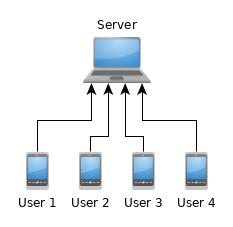
\includegraphics{school.png}


\chapter{Known issues and limitations}

\begin{itemize}
\item The end-user device must be cheaper than \$ 100.
\item The device will work in untrusted environment: at home, for example.
\end{itemize}


\chapter{Goals}

\begin{enumerate}
\item Provide a cheap replaceable device for educational purposes.
\item Determine the project hardware equpment and networking environment.
\end{enumerate}


\chapter{Scope of work}

\section{Requirements}

\begin{enumerate}
\item The end-user device must have a simple rollback functionality for
the cases of incorrect user exploitation.
\item The end-user device must have a limited access to the websites.
\item The end-user device must have application installation
functionality blocked.
\end{enumerate}

\section{Defintion of Done (artifacts)}

\begin{enumerate}
\item Report describing solutions for limiting access to websites and
3rd party software on end-user devices.
\item Provide simple device configuration tutorial in english
\textbf{or} spanish.
\end{enumerate}


\part{Project state}

\chapter{Overview}

\chapter{Server-side}

\chapter{Client-side}

Generally, standard parental control function is enough to provide the
necessary security level for children. Currently the configuration
process is manual and there is no way provided to ensure that multiple
devices will be configured alike.


\part{Project details}

\chapter{Server side}

It's advised to have as much functionality on server-side as possible
to reduce problems with client devices.


\section{Authentication}

There is software for WiFi HotSpots fencing called CoovaChilli:
http://coova.github.io/CoovaChilli/ . It's abandoned somehow but it's
the most functional solution for organizing fenced connection of
multiple users.


\section{Authorization}

Tasks like filtering the undesired traffic are also done better from
the server side - it'll be possible to avoid such problems like
adjusting tablets for this kind of work.


\section{Accounting}

If needed. WIP.


\chapter{End user side}

It's expected that the target audience is totally inexperienced with
computers so the less actions they will need to do to achieve the
desired result - the better.


\section{Access limiting}

Android's standard profiles and parental control function is enough to
limit the end-user access to programs and whitelisted websites.

The account of the device owner may be protected by graphical key
making it rather problematic to crack.

It should also be noted that modern Android versions have device control
feature that may prevent the unauthorized user from device reset -
in case the device reset is performed without correct password - the
device may turn into brick and become nearly irreparable (may be
solved only by reflashing new OS on device).

The setup is point-and-click as for now so it won't work in case of
hundreds and thousands of devices but there is some ways (like using
Termux with configuration deployment tools) which must be investiated
further.


\section{Authentication}

Done transparently when device is connected to HotSpot via MAC. The
authentication and authorization is performed by CoovaChilli software
on server side.


\section{Rollbacks}

Android's new filesystem F2FS has snapshot and rollback functionality
but it must be investigated if it's used by existing devices. The
rollb


\section{Upgrades}

WIP


\end{document}

